\documentclass{standalone}
\usepackage{tikz}
\usepackage{amsmath}

\begin{document}

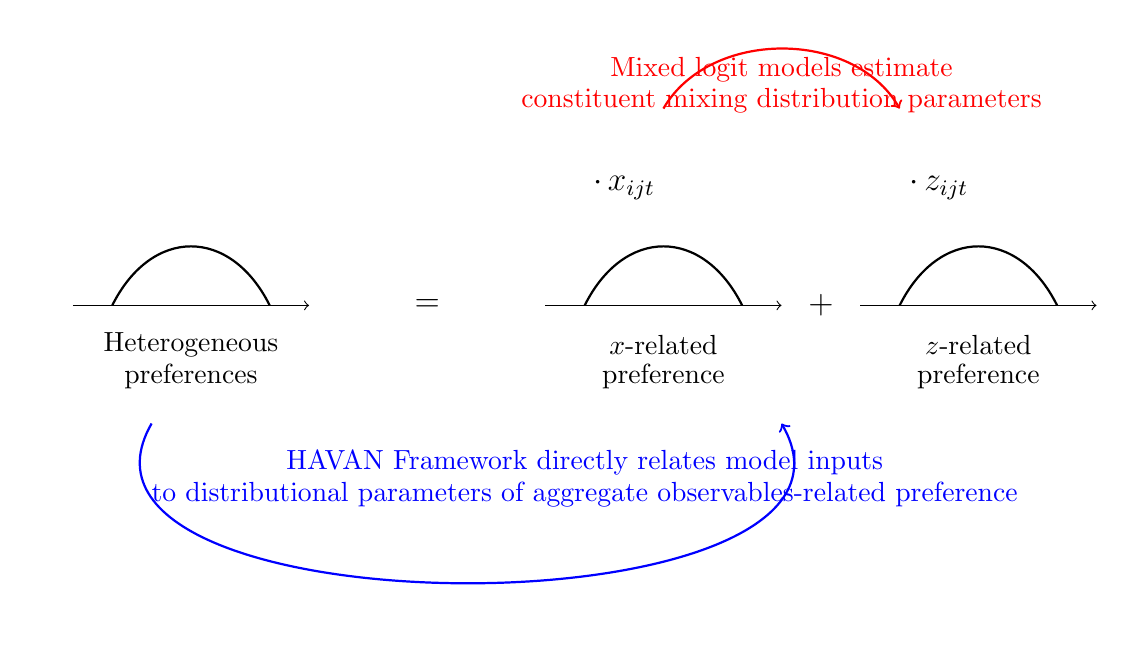
\begin{tikzpicture}

% Draw the distribution curves
\draw[thick] (0,0) .. controls (0.5,1) and (1.5,1) .. (2,0);
\draw[thick] (6,0) .. controls (6.5,1) and (7.5,1) .. (8,0);
\draw[thick] (10,0) .. controls (10.5,1) and (11.5,1) .. (12,0);

% Axes
\draw[->] (-0.5,0) -- (2.5,0);
\draw[->] (5.5,0) -- (8.5,0);
\draw[->] (9.5,0) -- (12.5,0);

% Labels
\node at (1,-0.5) {Heterogeneous};
\node at (1,-0.9) {preferences};
\node at (7,-0.5) {$x$-related};
\node at (7,-0.9) {preference};
\node at (11,-0.5) {$z$-related};
\node at (11,-0.9) {preference};

% Mathematical symbols
\node at (4,0) {\large $=$};
\node at (9,0) {\large $+$};

% Variables
\node at (6.5,1.5) {\large $\cdot \, x_{ijt}$};
\node at (10.5,1.5) {\large $\cdot \, z_{ijt}$};

% Arrows and text
\draw[->, red, thick] (7,2.5) to [out=60,in=120] (10,2.5);
\node[red] at (8.5,3) {Mixed logit models estimate};
\node[red] at (8.5,2.6) {constituent mixing distribution parameters};

\draw[->, blue, thick] (0.5,-1.5) to [out=-120,in=-60] (8.5,-1.5);
\node[blue] at (6,-2) {HAVAN Framework directly relates model inputs};
\node[blue] at (6,-2.4) {to distributional parameters of aggregate observables-related preference};

\end{tikzpicture}

\end{document}